% Underlying graph for minimum spanning tree (mst) example
% Redrawn from Figure 5.3 of the textbook ``Algorithms'' by Dasgupta

\documentclass[standalone]{beamer}

\usepackage{tikz}
\usetikzlibrary{positioning, mindmap}

\begin{document}

\begin{frame}{Example of Kruskal's Algorithm}
\begin{tikzpicture}[node distance = {1.0cm and 1.5cm}, 
  v/.style = {draw, circle},	% vertex
  kv/.style = {v, fill = teal},	% chosen by kruskal's algorithm
  ke/.style = {circle connection bar, brown, fill},	% kruskal edge
  nke/.style = {gray, dash pattern = on 5pt off 3pt, ultra thick},	% non-kruskal edge which would cause cycle
]
  \node (a) [v] {A};
  \node (c) [v, right = of a] {C};
  \node (e) [v, right = of c] {E};

  \draw (a) to node[above] {1} (c);
  \draw (c) to node[above] {3} (e);

  \node (b) [v, below = of a] {B};
  \node (d) [v, right = of b] {D};
  \node (f) [v, right = of d] {F};

  \draw (b) to node[below] {1} (d);
  \draw (d) to node[below] {4} (f);

  \draw (a) to node[left] {2} (b);
  \draw (c) to node[below] {2} (b);
  \draw (c) to node[right] {2} (d);
  \draw (e) to node[below] {3} (d);
  \draw (e) to node[right] {1} (f);

  \only<2->{\draw[ke] (a) to (c); \node [kv] at (a) {A}; \node [kv] at (c) {C};}
  \only<3->{\draw[ke] (b) to (d); \node [kv] at (b) {B}; \node [kv] at (d) {D};}
  \only<4->{\draw[ke] (e) to (f); \node [kv] at (e) {E}; \node [kv] at (f) {F};}
  \only<5->{\draw[ke] (a) to (b); \node [kv] at (b) {B};}

  \only<6->{\draw[nke] (b) to (c);}
  \only<7->{\draw[nke] (c) to (d);}

  \only<8->{\draw[ke] (c) to (e);}
\end{tikzpicture}
\end{frame}
\end{document}
